\subsection{Details of the Slingram Method}
\textit{Parts (a)-(c) are fairly technical and geared to train your math skills (e.g. by dealing with complex numbers). This is an important skill to have because it enables you to follow more advanced textbooks and papers. They also fill some gaps that we left open in our lecture. However, it is not needed to memorize any of the specific expressions derived. Only the techniques and underlying principles matter (e.g. it is useful to memorize how the phase angle of a complex number is defined.). If you get stuck at one part, move to the next one. Explicit solutions will be provided in class.}\\

\textbf{(a)} Show that the ratio of secondary over the primary voltage in the Slingram method can be expressed as:
$$
 \frac{V_{l3,s}}{V_{l3,p}} = -\frac{L_{12}L_{23}}{L_{13}L_{l2}}\left(\frac{i\omega \frac{L_{l2}}{R_{l2}}}{1+i\omega\frac{L_{l2}}{R_{l2}}}\right)
$$
by using Faraday's law of induction and expressions for for the currents in the loops derived in class.   
\ifanswers
    \begin{tcolorbox}[enhanced jigsaw,breakable,pad at break*=1mm,
    colback=blue!5!white,colframe=babyblueeyes,title=Solutions,
    watermark color=white]
   
    Using Faraday's law of induction we know that the primary voltage in coil 3 is
    $$V_{l3,p} = L_{13}\frac{dI_{l1}}{dt}$$
    and the secondary voltage is
    $$V_{l3,s} = L_{23}\frac{dI_{l2}}{dt}.$$
    We derived expressions for $I_{l1}$ and $I_{l2}$ in class:
    \begin{eqnarray*}
    I_{l1} &=& I_1e^{i\omega t} \\
    I_{l2} &=& \frac{-i\omega \frac{L_{l2}}{R_{l2}}}{1+i\omega \frac{L_{l2}}{R_{l2}}}\frac{L_{12}}{L_{l2}}I_1e^{i\omega t}.
    \end{eqnarray*}
    We now need to calculate the temporal derivatives of the electrical currents using $\frac{d}{dt}e^{i\omega t} = i\omega e^{i\omega t}$. Then the ratio of the primary and secondary potentials is straightforwardly calculated:
    $$
    %\frac{V_{l3,s}}{V_{l3,p}} = \frac{iL_{13}\omega I_1 e^{i\omega t}}{iL_{23}\omega \frac{-i\omega \frac{L_{l2}}{R_{l2}}}{1+i\omega \frac{L_{l2}}{R_{l2}}}\frac{L_{12}}{L_{l2}}I_1e^{i\omega t} } = \frac{L_{13}}{L_{23} \frac{-i\omega \frac{L_{l2}}{R_{l2}}}{1+i\omega \frac{L_{l2}}{R_{l2}}}\frac{L_{12}}{L_{l2}}}
    \frac{V_{l3,s}}{V_{l3,p}} = \frac{iL_{23}\omega \frac{-i\omega \frac{L_{l2}}{R_{l2}}}{1+i\omega \frac{L_{l2}}{R_{l2}}}\frac{L_{12}}{L_{l2}}I_1e^{i\omega t} }{iL_{13}\omega I_1 e^{i\omega t}} = \frac{L_{23} \frac{-i\omega \frac{L_{l2}}{R_{l2}}}{1+i\omega \frac{L_{l2}}{R_{l2}}}\frac{L_{12}}{L_{l2}}}{L_{13}} = -\frac{L_{12}L_{23}}{L_{13}L_{l2}}\left(\frac{i\omega \frac{L_{l2}}{R_{l2}}}{1+i\omega\frac{L_{l2}}{R_{l2}}}\right)
    .$$
\end{tcolorbox}
\fi

\textbf{(b)} Show that:
$$
 \left(\frac{i\omega \frac{L_{l2}}{R_{l2}}}{1+i\omega\frac{L_{l2}}{R_{l2}}}\right) = \left(\frac{1}{1+\alpha^2}(\alpha^2+i\alpha) \right)
$$
using the induction paramter $\alpha = \omega \frac{L_{l2}}{R_{l2}}$.
\ifanswers
    \begin{tcolorbox}[enhanced jigsaw,breakable,pad at break*=1mm,
    colback=blue!5!white,colframe=babyblueeyes,title=Solutions,
    watermark color=white]
    \begin{eqnarray*}
        \left(\frac{i\alpha}{1+i\alpha}\right) &=& \left(\frac{i\alpha}{1+i\alpha}\right)\left(\frac{1-i\alpha}{1-i\alpha}\right) \\
        &=&\left(\frac{i\alpha-i^2\alpha^2}{1-i^2\alpha^2}\right) \\
        &=&\left(\frac{\alpha^2+i\alpha}{1+\alpha^2}\right)
    \end{eqnarray*}
        
\end{tcolorbox}
\fi

\textbf{(c)} Show that:
$$
\phi_p - \phi_s = \frac{\pi}{2} + atan(\frac{\omega L_{l2}}{R_{l2}})
$$
whereas $\phi_p$ and $\phi_p$ are the phase differences relative to the primary loop.
\ifanswers
    \begin{tcolorbox}[enhanced jigsaw,breakable,pad at break*=1mm,
    colback=blue!5!white,colframe=babyblueeyes,title=Solutions,
    watermark color=white]
     From the lecture and (a) we know that $V_{l3,p} = L_{13}\frac{dI_{l1}}{dt} = i\omega I_1 e^{i\omega t}$ and $V_{l3,p} = iL_{23}\omega \frac{-i\omega \frac{L_{l2}}{R_{l2}}}{1+i\omega \frac{L_{l2}}{R_{l2}}}\frac{L_{12}}{L_{l2}}I_1e^{i\omega t}$. We use the induction parameter $\alpha = \omega\frac{L_{l2}}{R_{l2}}$ and rewrite as in the lecture:
     $$
     V_{l3,s} = iL_{23}\omega \frac{-i\omega \frac{L_{l2}}{R_{l2}}}{1+i\omega \frac{L_{l2}}{R_{l2}}}\frac{L_{12}}{L_{l2}}I_1e^{i\omega t} = i\omega\frac{L_{12}L_{23}}{L_{l2}}I_1e^{i\omega t} \left(\frac{1}{1+\alpha^2}(\alpha^2+i\alpha)\right) = c_1 \frac{1}{1+\alpha^2}(-\alpha+i\alpha^2)
     $$
     It is now clear what the real and imaginary components are. We can neglect the $e^{i\omega t}$ which is common in both primary and secondary induced voltage and will not lead to phase shifts in itself . Per definition (reassure yourself in the real/complex plane that this is the case): $\theta_s = atan(\frac{Im(V_{l3,s})}{Re(V_{l3,s})})$:
     $$
     \theta_s = atan\left(\frac{\frac{\alpha^2}{1+\alpha^2}}{\frac{-\alpha}{1+\alpha^2}} \right) = -atan(\alpha)
     $$
     This is the phase shift of the secondary component. Verify that this lead to the bounds derived in the lectures for the resistive and conductive limits. In $V_{l3,p}$ there is only an imaginary component and the real part is zero. Taking the limit  this results in the $\frac{\pi}{2}$ term.
\end{tcolorbox}
\fi
\textbf{(d)} (\textit{Already sketch out in class. This is a repetition for yourself.}) Suppose you have an idealised loop in the sub-surface (as sketched out in lecture) located in the center of an arbitrary profile. Sketch out the shape of the slingram anomaly with distance on the x-axis and the ratio $\frac{V_s}{V_p}$on the y-axis.
\ifanswers
    \begin{tcolorbox}[enhanced jigsaw,breakable,pad at break*=1mm,
    colback=blue!5!white,colframe=babyblueeyes,title=Solutions,
    watermark color=white]
    \begin{center}
        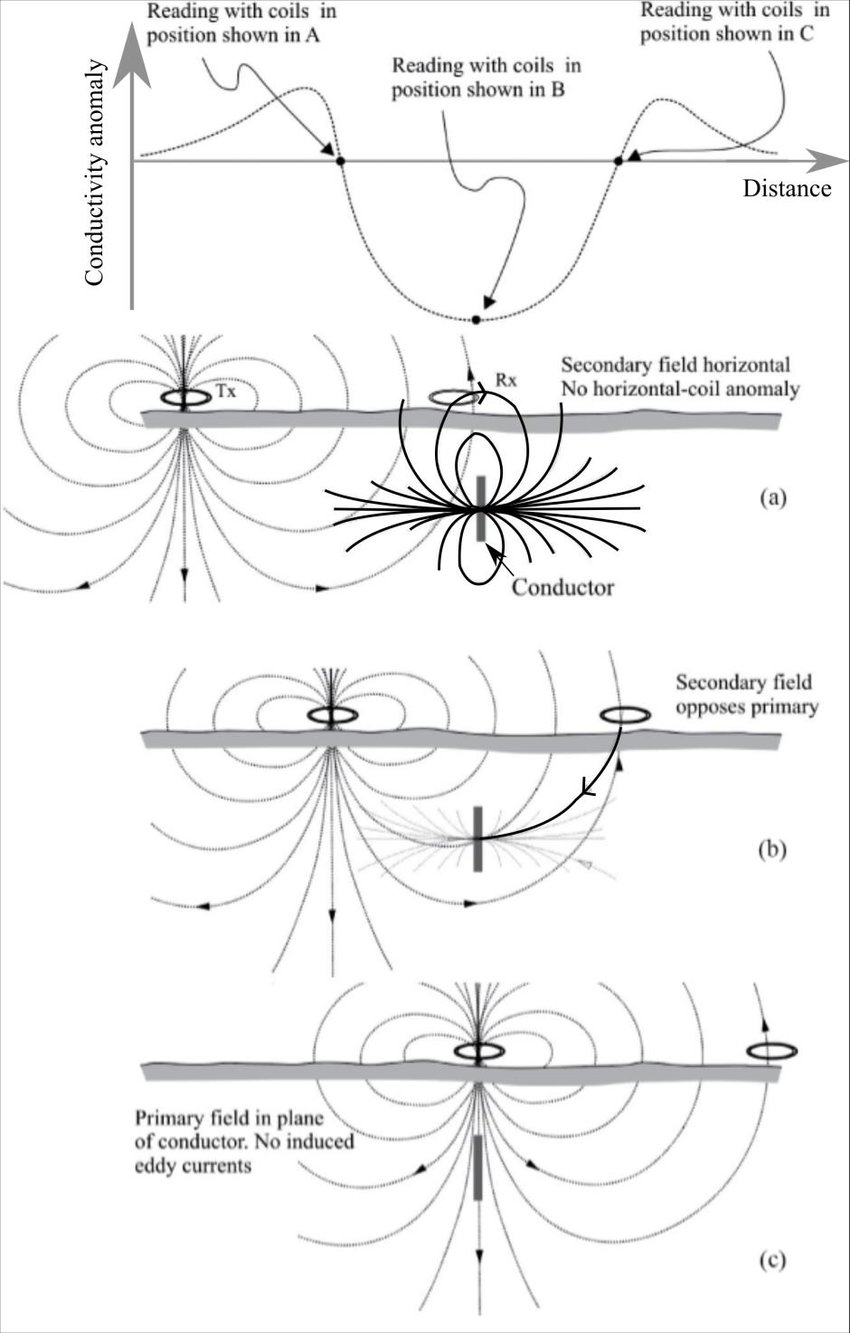
\includegraphics[width=12cm]{Includes/EMI/SlingrammAnomaly.jpg}
      \end{center}    
    \textbf{Solutions [Zylberman, 2018]:} In order to sketch out the anomaly you need to worry most about the coupling coefficients $L_{xx}$. They change in magnitude and sign as you go across this anomaly. With Rx and Tx on the left side of the anomaly the secondary magnetic field has the same direction in the receiver coil as the primary magnetic field. Hence the anomaly is positive. With the receiver coil directly above the target, the coupling coefficient turns to zero as field lines are parallel to the loop (i.e. no induction). With transmit and receiver coils bracketing the target, the secondary magnetic field is in opposite direction to the primary field and the anomaly is negative. The rest can be argued with symmetry reasons.
\end{tcolorbox}
\fi